% !TEX root = ../latex-faq-cn.tex
% Copyright (C) 2018 by latexstudio <http://www.latexstudio.net>
% 
% This program is free software: you can redistribute it and/or modify
% it under the terms of the GNU General Public License as published by
% the Free Software Foundation, either version 3 of the License, or
% (at your option) any later version.
% 
% This program is distributed in the hope that it will be useful,
% but WITHOUT ANY WARRANTY; without even the implied warranty of
% MERCHANTABILITY or FITNESS FOR A PARTICULAR PURPOSE.  See the
% GNU General Public License for more details.
% 
% You should have received a copy of the GNU General Public License
% along with this program.  If not, see <http://www.gnu.org/licenses/>.
% 

% !TEX root = ../latex-faq-cn.tex
% !TEX program = xelatex
% !TEX options = --shell-escape

\section{文档编辑}


\faq{\LaTeXTeX{} 教程}{latex-tex-tutorial}
lshort-zh 是一本比较薄的针对中文用户的 \LaTeX{} 入门教程,该教程已在发行版中,用户可以在命令行中执行
\begin{shcode}
  texdoc lshort-zh
\end{shcode}
来查阅。 \LaTeX wikibook 是
% \href{https://www.latex-project.org/help/books/}{https://www.latex-project.org/}
\url{https://www.latex-project.org/help/books/} 中列出的 \TeX{} and \LaTeX{} Books 之一,用户可访问
\url{https://en.wikibooks.org/wiki/LaTeX} 进行查阅。
除此之外,用户还可以购买胡伟、刘海洋等编著书籍,这里不再赘述。


\faq{关于 \LaTeX{} 的书籍}{latex-books}
\begin{itemize}
\item \LaTeX{} 入门,刘海洋, 电子工业出版社;
\item \LaTeX{2$\varepsilon$} 完全学习手册(第 2 版),胡伟,清华大学出版社;
\item \LaTeX{} 入门与提高(第二版) ,陈志杰等,高等教育出版社(注:此书出版逾十年,部分内容已经过时);
\item \LaTeX{} Beginner's Guide, Stefan Kottwit, Packt Publishing.
\end{itemize}


\faq{\LaTeX{} 支持中文有哪些方式,如何选择}{latex-chinese-how-to-choose}
历史上,\LaTeX{} 支持中文的方式包括中西文点点通、天元、CCT、CJK 等。目前流行的方式是使用 \CTeX{} 宏集,详情请见
\url{https://mirrors.tuna.tsinghua.edu.cn/CTAN/language/chinese/ctex/ctex.pdf}


\faq{关于教程,用户比较容易获取的有两个:lshort 和 \LaTeX{} wikibook。}{lshort-latex-wikibook}


% \faq{关于\TeX{}, Plain \TeX{} 及相关书籍}{tex-plain-tex-books}


% \faq{关于类型的书籍}{kind-related-books}


% \faq{关于其他TeX相关事项的书籍}{other-tex-books}


\faq{工具包文档}{package-document}

每个工具包自带的文档是最全面最权威的文档,一般可以通过 texdoc命令+工具包名的方式
找到相应工具包的文档。一些常用的工具包有不少爱好者写了自己使用过程中的经验,也可
以找来看看。


\faq{可免费提供的 \LaTeXTeX{} 书籍}{free-latex-tex-books}

\begin{itemize}
\item \LaTeX{} 常用数学符号
\item \LaTeX{} Note 包太雷
\item 一份不太简短的 \LaTeX{2e} 介绍
\item \TeX{} Live 指南 2018
\end{itemize}


\faq{获取在线帮助}{gain-online-help}

一般资料可以去 wikibook 上面查询,网址是
\url{https://en.wikibooks.org/wiki/LaTeX}。
提问可以先到 \LaTeX{} Stack Exchange 看看,网址是
\url{https://tex.stackexchange.com/}。


\faq{如何提出问题}{how-to-ask-questions}

在问问题的时候,要先自己尝试,先问自己如何解决,清晰有效的组织自己想问的问题,究竟想表达什么?没有人会为你不知所谓的问题
浪费时间,就算有人愿意理你,也会因为你的问题不清晰甚至完全无效的问题而伤透脑筋,为了自己,也为了别人,建议大家可以参考下
\href{https://www.jianshu.com/p/f96aa7f7bf59}{《提问的艺术》}这篇文字,清晰有效的提出自己的问题。迷你范例(MWE)
是为别人帮助解决你的问题提供最大化便利的有效手段之一。

最后,需要强调的是,我们愿意在我们的能力范围内为你的问题进行讨论,尽全力帮你解决问题,但这并不是我们的义务,应当尊重别人
拒绝提供帮助的权利。另外,在 QQ 群提出问题所使用的代码最好代码粘贴的网站,如
\href{https://paste.ubuntu.com/}{Ubuntu Pastebin}
或
\href{https://pastebin.com/}{Pastebin}
暂存,避免刷屏,影响效率。


\faq{如何制作一个迷你范例(MWE)}{how-to-make-MWE}
迷你范例即最小工作示例,英文简称 MWE,以下内容摘自刘海洋的《\LaTeX{} 入门》。

最小工作示例就是一个精简到最小长度的、可以说明所需问题的 \TeX{} 源文件。一方面,最小工作示例应该是一个完整的、可以直接
编译的文件,利用示例可以方便地再现遇到的问题,不需要添加额外的代码;另一方面,示例文件应该尽可能地短小(一个典型的 MWE
一般不超过 10 行),不包含额外的文件,也没有与问题无关的文字代码干扰相对错误的分析。完整的 MWE 应当包括如下信息:
\begin{itemize}
\item 编译环境,至少应当包括使用的操作系统(如 Windows,macOS,Ubuntu)、安装的发行版(如 \CTeX{},\TeX{} Liv
  e,\MacTeX{} )和使用的集成开发环境(IDE)或编辑器(如 WinEdit,TeXstudio,TeXshop)
\item 完整的编译命令,如使用的排版引擎(如 \LaTeX{},\XeLaTeX{})
\item 源文件使用的编码,不同的编辑器的默认编码设置不同,没有事先声明可能会造成复现 bug 困难或出现其他 bug
\item 完整的代码,但应尽量删除与错误无关的部分,即保证代码可以直接运行的前提下,删除所有与错误部分无关的内容和信息,
  足以重现出现的错误信息和问题即可。不要截图!使别人可以直接复制粘贴你的代码到编译器中,直接重现问题,而不是将时间浪费在
  码字上
\item 编译错误信息,或你发现与预期不符的 PDF 效果
\item 如使用了模板,还需附上模板的相关信息,如下载链接和使用说明
\end{itemize}


\faq{学习如何撰写 \LaTeX{} 类及工具包}{learn-how-to-write-latex-and-tools}

可以用命令行使用 |texdoc| 查看 clsguide,dtxtut,macros2e;classes,source2e,The TeXBook;expl3,interface3,
l3styleguide,source3(参考自\href{https://www.zhihu.com/question/27017364}{知乎})。以及《\LaTeX{2e}
文类和宏包学习手册》(胡伟,清华大学出版社)。


% \faq{MetaFont 和 MetaPost 教程}{metafont-metapost-tutorial}


% \faq{在线介绍:\LaTeX{}}{}


% \faq{在线介绍:Plain \TeX{}}{}


\faq{如何让参考文献满足国标GB7714-2015样式要求}{how-to-reference-GB}

有两种比较简单的方式。
\begin{itemize}
\item 利用 biblatex,一个典型示例如下
  \begin{texlist}
    \documentclass{ctexart}
    \usepackage[backend=biber,style=gb7714-2015]{biblatex}
    \addbibresource{bibfilename.bib}
    \begin{document}
    引用文献\cite{bibkey1,bibkey2}
    \printbibliography
  \end{document}
\end{texlist}
\item 利用 BiB\TeX,一个典型示例如下
  \begin{texlist}
    \documentclass{ctexart}
    \usepackage{gbt7714}
    \begin{document}
    引用文献\cite{bibkey1,bibkey2}
    \bibliography{bibfilename}
  \end{document}
\end{texlist}
\end{itemize}


% \faq{专家邮件列表}{}


% \faq{Pic\TeX{} 手册}{}


% \faq{基于 \TeX{} 系统的教程}{}


% \faq{排版教程}{}


\faq{关于 \TeX{} 的 Wiki 书籍}{tex-wiki-books}

\LaTeX{} wikibook 是 \url{https://www.latex-project.org/} 中列出的 \TeX{} and \LaTeX{} Books 之一,用户
可访问 \url{https://en.wikibooks.org/wiki/LaTeX} 进行查阅。


\faq{如何找到\ldots{}符号:}{how-to-find-symbols}

在 \LaTeX{} 中插入符号主要有两种思路。一种方式是加载符号宏包,利用宏包提供的命令插入符号;而对于 \XeTeX{} 引擎,目前
使用的多为 Unicode 编码的字体,直接加载 Unicode 字体,插入 Unicode 符号也是一种很好的办法。下面分别介绍:
\begin{itemize}
\item
  加载符号宏包:\emph{The Comprehensive LATEX Symbol List} 收录了上万文本或数学符号,在命令行中键入
  \begin{shcode}
    texdoc symbols-a4
  \end{shcode}
  即可打开该文档。此外,\url{http://detexify.kirelabs.org/classify.html} 提供了手写识别前述文档中所有符号的功能,
  十分便捷,它可直接符号所在宏包。在 macOS 下可以直接使用 detexify 的 app。另外
  \url{https://webdemo.myscript.com/views/main/math.html} 可将手写公式转化为 \LaTeX{} 或 MathML 代码

\item 插入Unicode符号:可以从各种Unicode码表或字符映射表中找到所需要的符号,查出
  其编码,加载支持该码位的字体,直接在编辑器中输入该符号即可。如果符号在源代码编
  辑器中无法正常显示,还可以使用\LaTeX{}的 |symbol| 命令输入。|symbol| 命令的具体
  用法是
  \begin{texlist}
    \symbol{<十进制编码>}
    \symbol{"<十六进制编码>}
    \symbol{'<八进制编码>}
    \symbol{`<字符形式(特殊符号须加转义符 \ )>}
    % hello 你好
  \end{texlist}

  \begin{texlist}
    \[
      P_{r,j}=\left\{\begin{array}{ll} 0 & \text{$r-j$ 为奇数},\\
                       r!\,(-1)^{(r-j)/2} & \text{$r-j$ 为偶数}.
                     \end{array}\right.
                 \]
  \end{texlist}
\end{itemize}

如果使用的TeXstudio软件想要查找某个符号,那么还可以拓展以下2个便捷的方式:
\begin{itemize}
\item 如下图点开1处的符号,再在2处选择符号类型,缩小查找范围,有运算符、关系、箭头、分隔符、Greek、Cyrillic等,再
  点击需要的符号加入到数学环境中去这样就插入完成了。

  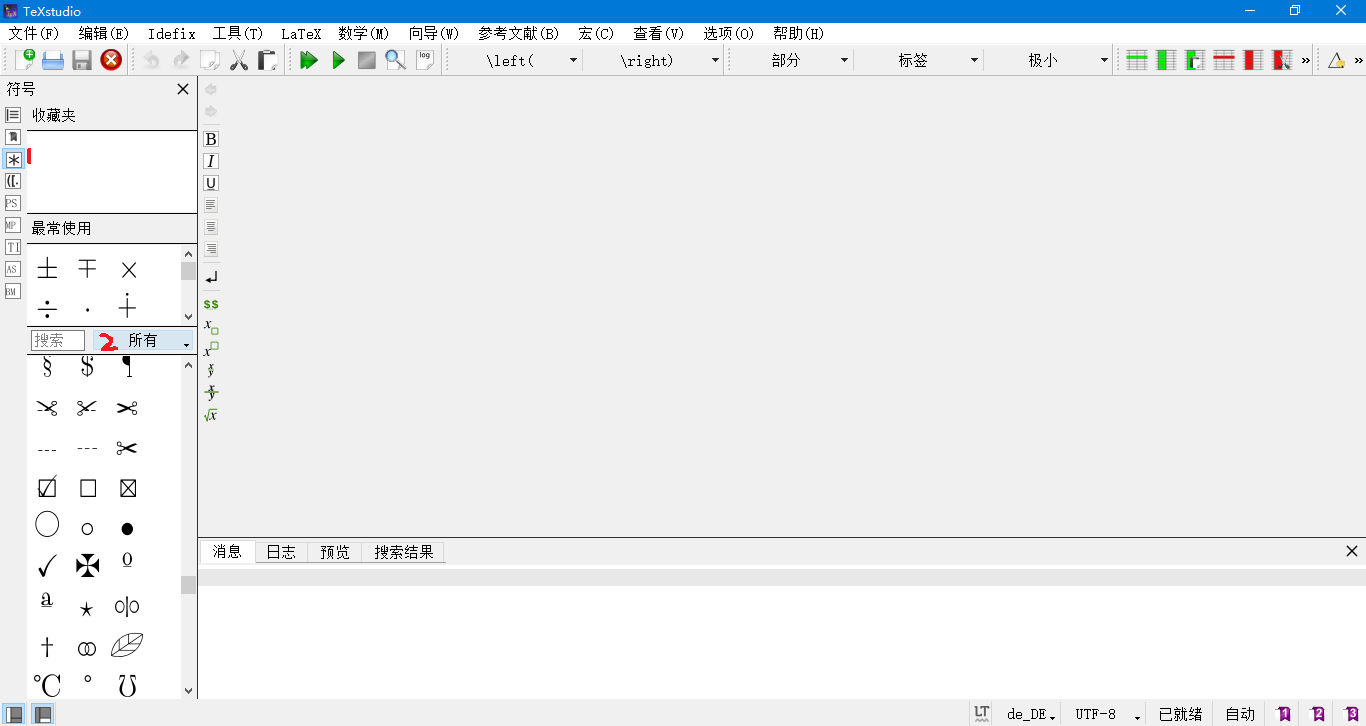
\includegraphics[width=0.9\textwidth]{../images/5.png}
\item 也可以手动输入,识别率不是特别高,可能需要多输入几次才会出来。设置如下:向导$\rightarrow$数学助手,手写输入完
  之后插入即可。

  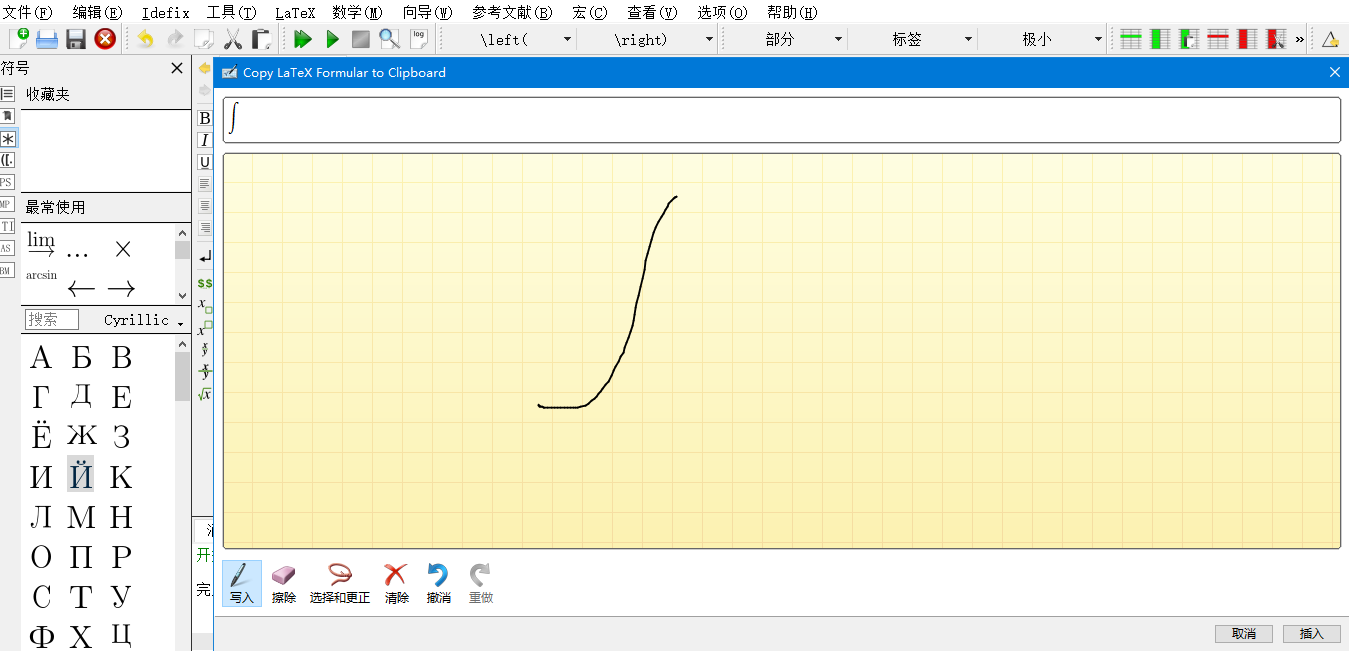
\includegraphics[width=0.9\textwidth]{../images/image.png}
\end{itemize}


% \faq{如何找到 FAQs}{}


\faq{如何控制章节编号的深度}{how-to-control-section-depth}

\LaTeX{} 标准文档类对章节划分了层级:
\begin{itemize}
\item 在 report/book 文档类里 part 为 $-1$,chapter 为 $0$,section 为 $1$,
  subsection为 $2$,subsubsection为 $3$,paragraph为 $4$,subparagraph为 $5$。
\item 在 article 文档类里 part 为 $0$,section 为 $1$,依此类推。
\end{itemize}

secnumdepth 计数器控制章节编号的深度,如果章节的层级大于 secnumdepth,那么章节的
标题、在目录和页眉页脚的标题都不编号(照常生成目录和页眉页脚),章节计数器也不计
数。可以用 |setcounter| 命令设置 secnumdepth 为较大的数使得层级比较深的章节也编号,
如设置为4令 |paragraph| 也编号;或者设置一个较小的数以取消编号,如设置
为-1 令 |chapter| 不编号。后者是生成不编号的章节的一个妙招,免去了手动使
用 |addcontentsline| 和 |markboth| 的麻烦。secnumdepth 计数器在 article 文档类里
默认为3(subsubsection 一级);在 report 和 book 文档类里默认为2(subsection 一级)。

下面给出一个具体的例子:

\begin{texlist}
  \documentclass{book}
  \setcounter{secnumdepth}{4}
  \begin{document}
  \part{Part}
  \chapter{Chapter}
  \section{Section}
  \subsection{Subsection}
  \subsubsection{Subsubsection}
  \paragraph{Paragraph}
\end{document}
\end{texlist}

控制目录页排版显示深度可以使用 |\setcounter{tocdepth}{2}|,此命令表示显示到三级标题。关于此问题的具体介绍可以参考
\href{https://blog.csdn.net/RobertChenGuangzhi/article/details/50480856}{该网页}。


\faq{如何下载 arXiv 上面的 \TeX{} 源文件}{how-to-download-arxiv-tex}
先访问 arXiv 上面的文章,在右边找到 Downloads $\rightarrow$ Other formats,点击进入下载页,点击 Download source。
将文件下载到本地后,重命名文件,文件后缀名是 .tar.gz。接下来解压缩 .tar.gz 文件,即可获得 \TeX{} 源文件。


\faq{Windows 系统下用 TeXstudio 打开中文编写的源文件遇到乱码怎么办}{windows-texstudio-chinese-GBK}

最简单的方法是借助 Notepad++ 等编辑器将文件转码为 UTF-8。如果没有 noteapd++,也可以直接使用 TeXstudio。
这里我们默认文件的编码是 GB2312。首先打开文件,在 TeXstudio 右下角找到 encoding 位置的内容,
有时系统显示为 ISO-8859-1。点击那里,进入 More encodings,在列表中点击 GB2312,然后点击按钮 view with。
正常来讲,乱码应该都会消失。 接下来,继续进入 More encodings,在列表中点击 UTF-8,然后点击按钮 change to。
经过这些操作,源文件就重新变成了 UTF-8 编码。


\faq{如何在listing抄录环境中显示公式}{how-to-listing-show-equations}

有时对抄录环境中的代码进行说明时,要用显示公式,这时只要进选项texcl设为true即可。

\begin{texlist}
  \begin{lstlisting}[
    numbers=left,
    upquote=true,
    basicstyle=\ttfamily,
    texcl=true,
    language=Python
    ]
    #Generates Graphs $G^{(12)} ---  G^{(17)}$
    sGL6=['E@QW', 'EHQW', 'E@`w', 'E@]o', 'E@Rw', 'EAMw']
    GL=[Graph(s) for s in sGL6]
  \end{lstlisting}
\end{texlist}
% 
%  % \begin{figure}
%  %   \centering
%  %   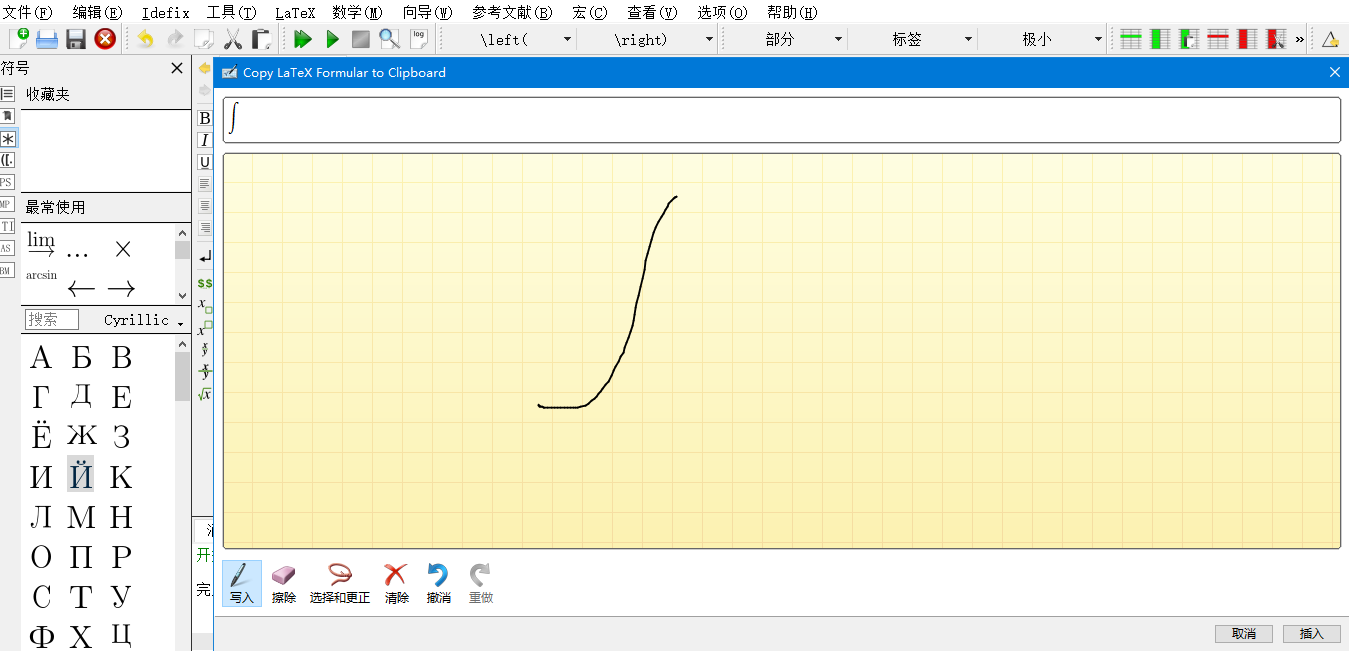
\includegraphics{https://images-cdn.shimo.im/LttXT6sECbcak9Qi/image.png!thumbnail}
%  %   \caption{图片}
%  % \end{figure}
% 

或者设置mathescape~选项为true。

\begin{texlist}
  \begin{lstlisting}[mathescape=true]
    if foo
    list= { $S_1,S_2,S_3$ }
  \end{lstlisting}
\end{texlist}


% \faq{能不能介绍一下排版试卷的方法与技巧,比如选择题,密封线设置等。}{how-to-latex-papers}


\faq{一个文档,如何在不同部分使用不同的页眉页脚}{how-to-set-different-geometry}

参考 geometry 宏包的自定义命令。比较常用的有如下四个命令
\begin{texlist}
  \newgeometry{<options>}
  \restoregeometry
  \savegeometry{<name>}
  \loadgeometry{<name>}
\end{texlist}
具体可参见该宏包的说明文档。


\faq{如何给中文文本加注音符号?}{how-to-pinyin}

xpinyin 宏包。


% \faq{在book类文档中边注用什么宏包?边注的宽度能调整吗?}{book-geometry}


% \faq{如何使用ctex相关类或者宏包制定章节样式,目录样式?}{ctex-tableofcontents}


% \faq{如何给章节标题,目录列表加盒子边框?}{}


\faq{如何使用带圈数字?}{how-to-use-circle-number}

注:百分号后的内容在导言区使用。
\begin{itemize}
\item 有序列表
  \begin{texlist}
    % \usepackage{enumerate,pifont}
    \begin{enumerate}[label={\ding{\value*}},start=172]
    \item 第一
    \item 第二
    \end{enumerate}
  \end{texlist}
\item 脚注中使用
  \begin{texlist}
    % \usepackage{pifont}
    % \RenewDocumentCommand{\thefootnote}{}{
    % \ding{numexpr171+\value{footnote}}
    % }

    \footnote{text}
  \end{texlist}
\end{itemize}


\faq{如何改变列表标签样式,行距,缩进等各种相关间距?}{how-to-change-list-style}

enumitem 宏包


\faq{换行与换段的区别,有几种方式?}{change-line-paragraph}

换行是 |\\| 换段是 |\par|,或者空一行。
换行与分段最大的区别在于语义上是否形成一段完整的阐述、叙述,多读两遍你写的文字,如果你觉得问题没有叙述完,那么应该用换行,
反之则应该用分段。


\faq{在使用较早版本的CTeX里面附带的WinEdt出现打不开UTF-8编码文档的情况,如何处理?}{early-version-ctex-winedit-utf8}

使用记事本之类文本编辑器打开,转换编码方式另存一份即可。有时候需要注意BOM问题,一般没啥问题。


\faq{如何改变计数器样式为中文数字、罗马数字、阿拉伯数字或拉丁字母?}{how-to-change-listing-number}

可以通过重定义命令的方式修改默认的计数器样式,例如
\begin{texinlist}
  \renewcommand{\thechapter}{\Roman{chapter}}
\end{texinlist}
会将章序号计数器改为大写罗马数字计数形式。更多对应关系如下所示:

\begin{table}[h]
  \centering
  \begin{tabular}{cc}
    |\arabic| & 阿拉伯数字 \\
    |\alph| & 小写英文字母,数值应小于27 \\
    |\Alph| & 大写英文字母,数值应小于27 \\
    |\chinese| & 中文小写数字,需要调用\CTeX{}宏包 \\
    |\roman| & 小写罗马数字 \\
    |\Roman| & 大写罗马数字 \\
    |\fnsymbol| & 脚注标识符,数值应小于10
  \end{tabular}
\end{table}

详情可以参阅刘海洋、胡伟等编写的相应书籍,也可以查阅Wiki百科。


\faq{列表环境 (enumerate/itemize/description)的条目间距太大了,怎么改小一些?}{how-to-change-listing-linespace}

可以使用 paralist 宏包,它提供了一系列压缩了行间距的列表。对应的环境名称分别是 compactenum/compactitem/compactdesc,
也可以使用 enumitem 宏包修改三个列表环境的格式。


\faq{列表的条目项内容很短,可以让他们在一行内排版么?}{listing-short-oneline}

可以使用 paralist 宏包,这个宏包提供了 inparenum/inparitem/inpardesc 环境,可以在行内输出列表内容;
也可以带上 inline 选项使用 enumitem 宏包,可以使用带*形式的三个列表环境,即在行内输出列表内容。


\faq{enumerate宏包修改列表标签格式很方便,但是这个宏包和enumitem宏包冲突,有什么解决办法么?}{enumerate-fight-enumitem}

如果只是需要使用这种短标签表示方法,利用enumitem宏包同样能够做到,只需要带上shortlabels选项加载enumitem宏包即可。
同时,enumitem宏包提供了自定义短标签名称和格式的宏命令,你也可以自己定义一些有趣的标签形式。


\faq{如何使用带圈数字作为 enumerate 列表的标签?}{circle-number-enumerate}

\LaTeX{} 自带一个带圈字符的命令 |\textcircled|,不过,这个命令的排版效果非常差,几乎很少有人会直接使用。
带圈数字可以通过unicode字符实现,也可通过pifont宏包中|ding|命令实现(但是只能用到10以内的数字),
甚至可以通过tikz 自己绘制一个。使用带圈数字做enumerate的标签,可以通过 enumitem 宏包设置。
这里给出一个使用 unicode 字符实现带圈数字的方法,并将其应用于enumerate 的标签。

\begin{texlist}
  \documentclass{article}
    \usepackage{xeCJK,xunicode,calc}
    \usepackage[shortlabels]{enumitem}
    \newcommand{\Cnum}[1]{%
    \ifnum #1<21
      \edef\a{\the\numexpr #1+9311}
    \else
      \ifnum #1<36
        \edef\a{\the\numexpr #1+12860}
      \else
        \ifnum #1<51
         \edef\a{\the\numexpr #1+12941}
        \else
          \PackageError{your package}{Number too large}{}
        \fi
      \fi
    \fi
    {\CJKfontspec{Noto Serif CJK SC}\fontspec{Noto Serif CJK SC}\symbol\a}}
    \SetEnumerateShortLabel{o}{\protect\Cnum{\arabic*}}
    \begin{document}
    \Cnum{12} \Cnum{32} \Cnum{46} 
    
    \begin{enumerate}[o]
    \item The first item.
    \item The second item.
    \item The Third One.
    \end{enumerate}
  \end{document}
\end{texlist}


\faq{如何给目录中的章节都带上引导点来连接页码?}{tableofcontents-dotdotdot}

其实级别较高的章节结构,如book/report中的chapter和arcticle中的section,是不需要这种引导点来连接页码的,有这种需求
的多是受Microsoft Word的影响。如果一定要这种引导点,可以在导言区增加这样一段代码。
\begin{texlist}
  \makeatletter
  \def\@bfdottedtocline#1#2#3#4#5{%
  \ifnum #1>\c@tocdepth \else
  \vskip \z@ \@plus.2\p@
  {\leftskip #2\relax \rightskip \@tocrmarg \parfillskip -\rightskip
  \parindent #2\relax\@afterindenttrue
  \interlinepenalty\@M
  \leavevmode \bfseries
  \@tempdima #3\relax
  \advance\leftskip \@tempdima \null\nobreak\hskip -\leftskip
  {#4}\normalfont\nobreak
  \leaders\hbox{$\m@th
  \mkern \@dotsep mu\hbox{.}\mkern \@dotsep
  mu$}\hfill
  \nobreak
  \hb@xt@\@pnumwidth{\hfil\normalfont \normalcolor #5}%
  \par}%
  \fi}
  \renewcommand*\l@section{\@bfdottedtocline{0}{0em}{1.5em}}
  \makeatother
\end{texlist}
当然,最后一句应根据实际的文档类型来重定义 |\l@chapter| 或 |\l@section|。

也可以借助于 tocloft 宏包简单实现这一功能。
\begin{texlist}
\usepackage{tocloft}
\renewcommand{\cftsecleader}{\cftdotfill{\cftdotsep}} % article 的目录中,section也加点。
% \renewcommand{\cftchapleader}{\cftdotfill{\cftdotsep}} % book/report 的目录中,chapter也加点。
\end{texlist}


% \faq{如何临时切换页面大小?}{}


\faq{没有编号的章节标题如何添加到目录里?}{no-number-chapter-tableofcontents}

使用 |\addcontentsline{toc}{<level>}{<title>}|;举个例子:
\begin{texlist}
  \section*{译者序}\addcontentsline{toc}{section}{译者序}
\end{texlist}
这样在目录中译者序是没有编号的,对应等级是section,标题是译者序。参考:《lshort》目录章节。


\faq{怎样定义“第几页/共几页”的页码样式?}{how-to-define-pagenumber}

可以调用末页标签宏包 lastpage,并将页码设置如下:
\begin{texlist}
  第 \thepage 页 / 共 \pageref{LastPage} 页
\end{texlist}

如果不想调用这个宏包,还可以自己DIY,虽然ugly,但是可以达到目的 ):在文档末尾设置一个标签,
例如在 |\end{doucument}| 前加一句 |\label{AllPage}|,然后将页码设置为:
\begin{texlist}
  第 \thepage 页 / 共 \pageref{AllPage} 页
\end{texlist}


\faq{超链接如何断行?}{url-how-to-multilines}

先写
\begin{texlist}
  \PassOptionsToPackage{hyphens}{url}
\end{texlist}

再写
\begin{texlist}
  \usepackage{hyperref}
\end{texlist}


\faq{如何在axmath转换代码到 \LaTeX ?}{how-to-axmath-exchange-to-latex}

点击下图中第10个按钮,或者键入Ctrl+Tab即可将数学公式转换为\LaTeX{}代码,复制即可。

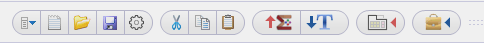
\includegraphics[width=0.9\textwidth]{../images/amxmath_texstudio}


\faq{双栏文档中,如何可以让左边先写完,然后再切换到右边,而不是左右一样长?}{twocolumn-left-first}

如果是采用文档类 twocolumn 选项实现的双栏模式,正文的排版就是先将左边排完,再从右边开始排。而采用
multicol 宏包的 muticols 环境则是左右两边底部对齐的。


\faq{如何输入中文破折号?}{input-chinese---}

输入法输入咯,英文的破折号 --- 用于中文不合适。


\faq{input和include有何区别?}{input-include-difference}

\begin{itemize}
\item |\include| 在读入文件之前会另起一页。|\input| 命令纯粹是把文件里的内容插入
\item |\include| 不可用于导言区,而且导言区使用了 |\includeonly| 命令后,
  |\include| 仅会引入由 |\includeonly| 指定的文件。
\item |\include| 引入的文件中,不可以再次使用 |\include| 命令。
\end{itemize}


\faq{subfiles有什么用?}{subfiles-usage}

详细功能可以查看此宏包自带的文档。编辑由一个主文档若干个子文档构成的多文档项目时使用此宏包会更方便。用户可以正常编译使用
|\input| 导入子文档的主文档,也可以直接编译子文档本身,此时子文档使用跟主文档相同的导言区而成为完整的一份\TeX{}文档。


% \faq{如何使用latexmk编译文档?}{}


% \faq{定理环境要怎么使用?}{}


% \faq{算法环境如何使用?}{}


% \faq{在lstlisting环境中如何输出破折号?}{}


% \faq{minted里面Tab键为什么会输出成\^{}\^{}T,如何解决?}{}


% \faq{一段代码粘贴到TeXstudio里面就没有了缩进,如何解决?}{}


% \faq{在\LaTeX{}或Tikz中,能否输入随机且字数随机可控的文字?}{}


\faq{如何输入罗马数字等?}{how-to-input-roman-numbers}

一种方式是定义宏显示罗马数字,代码如下:
\begin{texlist}
  \newcommand{\Myroman}[1]{\romannumeral #1}
  \newcommand{\MyRoman}[1]{\expandafter\@slowromancap\romannumeral #1@}
\end{texlist}
正文中使用
\begin{texlist}
  \MyRoman{3} \Myroman{5}
\end{texlist}

另一种投机取巧的方式是你可以先定义一个counter,然后给这个counter的数值设置成需要表达的数值,
再用 |\Roman| 或 |\roman| 显示这个计数器。举例如下:
\begin{texlist}
  \newcounter{romannum}
  \newcommand{\MyRoman}[1]{\setcounter{romannum}{#1}\Roman{romannum}}
  \newcommand{\Myroman}[1]{\setcounter{romannum}{#1}\roman{romannum}}
\end{texlist}
使用方法相同。


\faq{如何在等号中插入问号?}{how-to-input-.-in-questionmark}

\begin{texlist}
  \stackrel{?}{=}
\end{texlist}


\faq{如何在插入的图片上标记引注?}{input-mark-in-pictures}

可以看看overpic之类的宏包。


\faq{如何让一个很长很长的字符串(中间不带空格)自动换行?}{how-to-disable-long-string-multilines}

了解下分词断行机制就不会有此问题了。


% \faq{\cs{bf}、\cs{sf}、\cs{it}、\cs{sl}这些命令都很短小,为什么不建议继续使用了?}{}


% \faq{如何自动化打包 \LaTeX{} 文档发送给别人以确保宏包、字体是完整的,便于他人顺利编译、减少麻烦。}{}


% \faq{如何编译网站上下载的他人的模板,一般是不知道对应的编译器应该选择什么,还有编译顺序是什么,
% 希望在提供模板的同时说明应该如何编译。}{}


% \faq{我以book文档类为基础新写一个文档类,book文档类的选项会自动适用于我新建的文档类么?}{}


% \faq{\cs{def} 和 \cs{newcommand} 有什么区别,我创建新命令的时候究竟应该用哪个?}{}


\faq{怎样创建一个带*的命令?}{newcommand-with-*}

有以下几种方法:
\begin{itemize}
\item 最基本的方法,使用 \LaTeX{} 内部命令 |\@ifstar| 判断
\begin{texlist}
    \makeatletter
    \newcommand{\mycommand}{%
      \@ifstar
        \mycommandStar%
        \mycommandNoStar%
    }
    \makeatother
    \newcommand{\mycommandStar}{starred version}
    \newcommand{\mycommandNoStar}{normal version}
\end{texlist}
\item 比较简单的方法,使用 ifthen 宏包
\begin{texlist}
    \usepackage{ifthen}
    \newcommand{\mycommand}[1]{\ifthenelse{\equal{#1}{*}}%
      {\mycommandStar}%
      {\mycommandNoStar{#1}}%
    }
    \newcommand{\mycommandStar}{starred version}
    \newcommand{\mycommandNoStar}[1]{normal version}  
\end{texlist}
\item 使用\LaTeX{3}的机制
\begin{texlist}
    \usepackage{xparse}
    \NewDocumentCommand\mycommand{s}{%
      \IfBooleanTF#1%
        {starred version}%
        {normal version}%
    }
\end{texlist}
\end{itemize}


% \faq{类似 \cs{macro[<option1>][<option2>]\{<arg>\}} 这样的宏命令,当我只使用一个可选参数时,\LaTeX{}把它看做哪个参数?\LaTeX{}会自动判断么?}{}


\faq{\cs{newcommand} 创建的命令,仅有第一个命令可以成为可选参数,如果我想创建具有两个可选参数的命令,应该如何去写?}
{newcommand-multi-optional}

可以用一个小把戏实现:
\begin{texlist}
  \newcommand{\mycmd}[1][option1]{%
    \def\ArgI{{#1}}%
    \mycmdoptii
  }
  \newcommand\mycmdoptii[1][option2]{%
    ...
  }
\end{texlist}

或者使用\LaTeX{3}的机制:
\begin{texlist}
  \usepackage{xparse}
  \NewDocumentCommand\mycmd{O{option1} O{option2} m}{%
    #1#2#3
  }
\end{texlist}


% \faq{有些命令的参数是使用 () 扩起来的,这类命令是如何定义的?}{}


\faq{我想新建一个带有可选参数的命令,可选参数的缺省值与必选参数值一样,这样的命令如何创建?}{}

第一种方法:
\begin{texlist}
  \newcommand{\mycmd}[2][\DefaultOpt]{%
    \def\DefaultOpt{#2}%
    optional arg: #1,  mandatory arg: #2%
  }
\end{texlist}

第二种方法:
\begin{texlist}
  \def\mycmd{\futurelet\testchar\WithOptCmd}
  \def\WithOptCmd{%
    \ifx[\testchar 
      \let\next\OptCmd 
    \else 
      \let\next\NoOptCmd 
    \fi\next}
  \def\OptCmd[#1]#2{optional arg: #1,  mandatory arg: #2}
  \def\NoOptCmd#1{optional arg: #1,  mandatory arg: #1}
\end{texlist}


\faq{想用minted包写文档,怕别人用不来不会设置-shell-escape咋办}{}

教给别人怎么用,或者不用这个宏包。


% \faq{如何给整个页面加边框?}{}


\faq{每一部分第一段段首如何空两格,区别于下面段落的自动换行。}{}

使用 |\usepackage{indentfirst}|


% \faq{如何在section中使用box}{}


% \faq{\cs{lstinputlisting}在\XeLaTeX{}下如何支持中文?}{}


% \faq{Excel里的矢量图怎么存为eps并插入\TeX{}中?\& Matlab 导出图片无白边?}{}


% \faq{如何结合使用 Pandoc 和 \LaTeX{},提高文档编写效率?(或如何结合使用 Markdown 和 LaTeX?)}{}


% \faq{\cs{label\{key\}}可以用中文吗,如\cs{label\{第一章\}}}{}


% \faq{如何将算法代码的行编号放到外边框的里面?}{}


% \faq{如何编辑页眉和页脚,添加页码}{}


% \faq{\LaTeX{}写毕业论文时,直接写编译速度慢,用dvi会不会简便些?}{}


\faq{文字用 \cs{underline} 加了下划线后为什么没法换行?}{underlinebox}

\cs{underline}与 \cs{hbox}、\cs{mbox}等均工作在\textit{受限的水平模式(Restricted
  horizontal mode)}下,不能自动换行。

可以尝试使用 ulem 宏包的\cs{uline}或 XeCJK 宏包的\cs{CJKunderline}实现换行,但这
两者目前对math mode(尤其是displaystyle的math mode)支持有限。

\begin{reference}
\item \url{https://tex.stackexchange.com/questions/13177/what-are-vertical-and-horizontal-modes}
\end{reference}

% \faq{如何使用带圈数字做脚注编号?}{}


% \faq{怎样判断当前页是奇数页还是偶数页?}{}


% \faq{如何加粗Listing中的一行文本?}{}


% \faq{如何根据不同的编译引擎选择执行不同的宏命令?}{}


% \faq{我怎么能把页码改成以三位数字(前导的0也显示出来)表示?}{}


% \faq{標點符號如何分類設置樣式?比如逗號、句號、頓號等設爲一類,歎號、問號設爲一類,引號、書名號設爲一類,等等。}{}


% \faq{请问交叉引用用\cs{ref\{\}}引用的表格,图片,在PDF上点击数字时没有反应,不能跳转到相应的表格、图片位置,
% 生成的目录点击时也跳转不到指定的页码,在书上没有查到原因,我用的\TeXLive{} 2017+TeXstudio,是设置的问题还是其他问题?}{}
